\section {Arhitectura sistemului}

Sistemul prezentat presupune atat o partare hardware, cat si una software. Hardwareul realizeaza adaptarea dintre terminalul analog POTS si placa digitala de dezvoltare Raspberry Pi, iar ca software am folosit NodeJS pentru server si Android pentru a implementa un client al serverului

\subsection {Raspberry Pi HUT}

Pentru a proiecta un \acrfull{pcb} am folosit softwareul Fritzing. Acesta permite proiectarea schemei electrice si ulterior trasarea conexiunilor pe layoutul fizic al placii.

\begin{figure}[h!]
  \centering
  \fbox {
    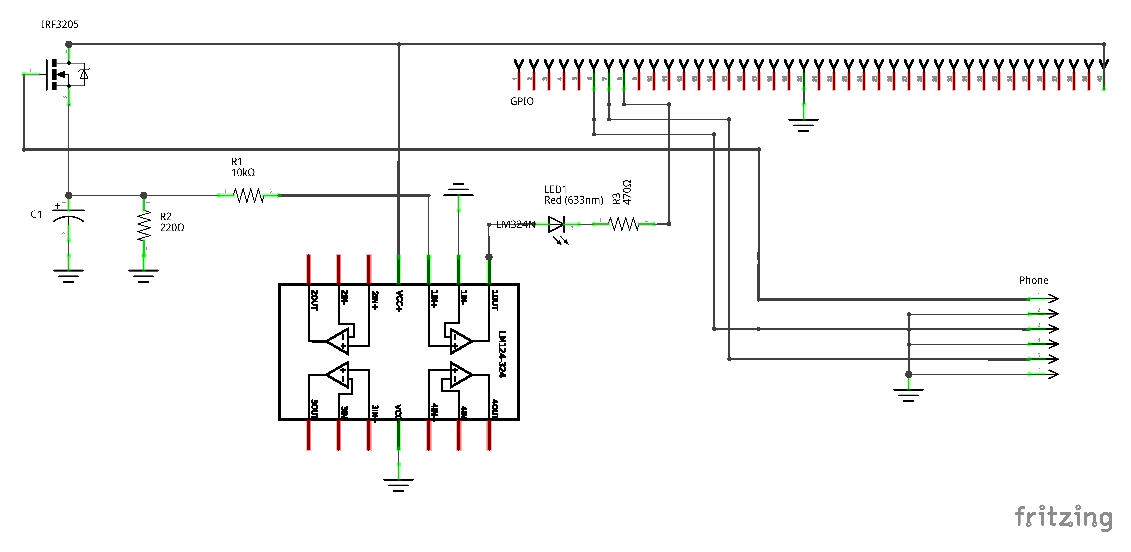
\includegraphics[width=0.6\textwidth]{04/04_schema_electrica_hut.pdf}  
  }
  \caption{Schema electrica HUT Raspberry PI}
\end{figure}

Actionarea butoanelor terminalului \acrshort{pots} se realizeaza cu ajutorul unor opto-cuploare, izoland circuitul interfonului care este proiectat pentru a functiona cu spike-uri de pana la 90V de circuitul Raspberry Pi.

Detectarea unui apel este realizata prin legarea unui \acrfull{mosfet} la bornele difuzorului terminalului \acrshort{pots} si inserierea cu un amplificator operational in regim de comparator cu referinta de 0.1V. Am folosit de asemenea si un Filtru Trece Jos deoarece terminalul este sensibil la zgomote, declansand accidental notificarea.

\begin{figure}[h!]
  \centering
  \fbox {
    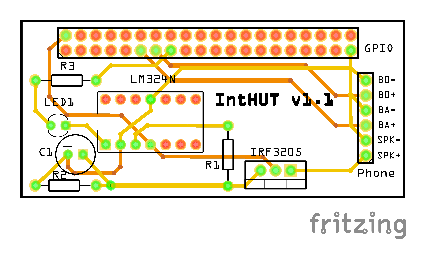
\includegraphics[width=0.6\textwidth]{04/05_schema_pcb_hut.pdf}  
  }
  \caption{Schema electrica HUT Raspberry PI}
\end{figure}

\subsubsection {Optocuploare homemade}

Datorita crizei globale de semiconductori, o placuta breakout care care include doua optocuploare costa aproximativ 50 RON. Considerand simplitatea functionarii acestui circuit, am decis sa construiesc propria solutie, folosind componetele de baza: un rezistor pentru limitat curentul, un LED si un fotorezistor. Platforma Raspberry Pi furnizeaza pinilor sai \acrshort{gpio} 3.3V si un curent maxim de 16mA, iar un LED rosu are o cadere de tensiune de 2.4V:

\begin{center}
\begin{gather*}
I_{GPIO} =10\ mA=10^{-2} A\\
V_{R} =V_{GPIO} -V_{LED} =3.3V-2.4V=0.9V\\
I_{GPIO} =\frac{V_{R}}{R} \ sau\ R=\frac{V_{R}}{I_{GPIO}} =\frac{0.9V}{10^{-2}A} =90\Omega
\end{gather*}
\end{center}

Am lipit rezistorul de 90$\Omega$ la anodul ledului si am incastrat LED-ul impreuna cu fotorezistorul intr-o incinta fara lumina.

\begin{figure}[!ht]
\begin{center}
  \subfloat[Schema optocuplor \cite{OptocouplerCircuitsToday}]{\label{fig:optoa}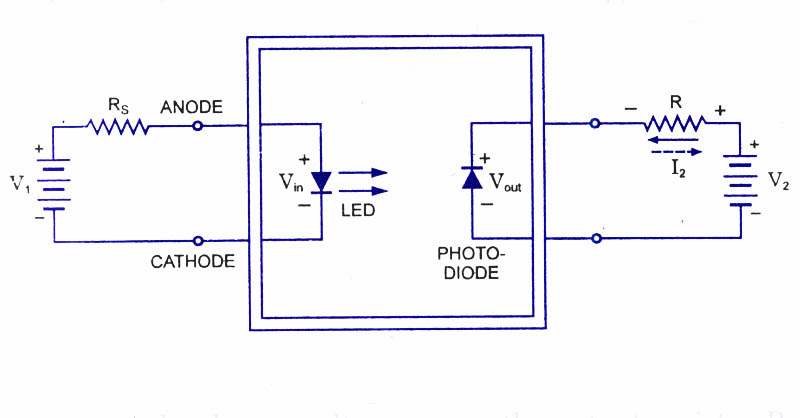
\includegraphics[width=\doublefigure]{04/01_optocoupler_scheme.jpg}}
  \subfloat[Componenta realizata manual]{\label{fig:optob}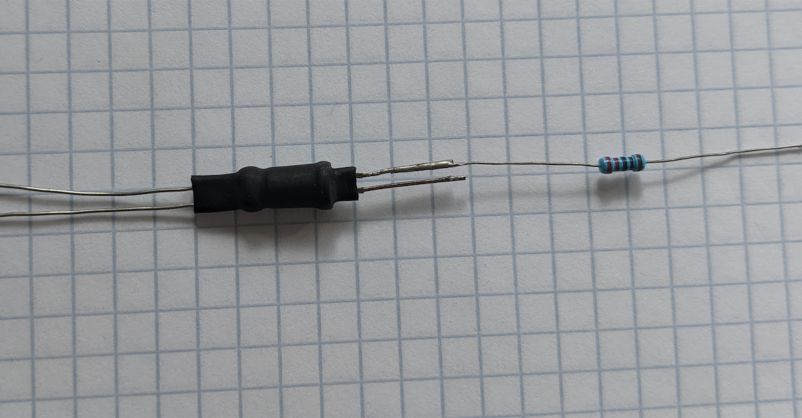
\includegraphics[width=\doublefigure]{04/02_optocoupler_assembly.png}}
  \caption{Schema electrica optocuplor (a) si rezultat ansablu (b)}
  \label{fig:opto}
\end{center}
\end{figure}


Deoarece aveam nevoie sa scurtcircuitez un contactor pe partea terminalului \acrshort{pots} am omis rezistenta legata fotorezistorului. Atunci cand ledul este aprins, rezistenta fotorezistorului scade, comportandu-se aproape ca un conductor ideal, atingand lamelele contactorului corespunzator receptorului.

\subsection {Webserver NodeJS}

NodeJS este un

\subsubsection {Autentificare}

Pentru autentificarea si validarea credentialelor utilizatorilor, am ales metoda \acrfull{jwt}, un standard open source in industrie conform RFC 7519. In cea mai compacta forma a sa, acesta este compus din trei parti, despartite prin caracterul ".":

\begin{enumerate}
  \item Header (algoritm si tipul tokenului)
  \item Continut (id utilizator, nume, rol)
  \item Semnatura
\end{enumerate}

Semnatura este calculata cu ajutorul unui algoritm simetric de hashing \acrfull{hs256} si a unei chei private aplicat pe forma codata in baza 64 a continutului si metadatelor despre token (expirare, emitator, audienta, subiect). Toate cele trei informatii sunt apoi concatenate cu caracterul "." intre, constituind forma finala ce va trimisa clientului. Clientul va folosi acest token in comunicatiile ulterioare cu serverul, acesta folosindu-se de mesaj, semnatura acestuia si cheia privata pentru a determina daca a fost sau nu modificat pe parcurs.

Folosirea algoritmului simetric implica faptul ca secretul este utilizat atat pentru generarea de tokenuri, cat si pentru validarea lor. In cazul aplicatiei din lucrare, aceasta nu este o problema, deoarece ambele metode ruleaza in interiorul aceluias proces, fara sa expuna aplicatia la vulnerabilitati.

Un avantaj al \acrshort{jwt} este faptul ca serverul nu trebuie sa intretina starea unei tabele de sesiuni a utilizatorilor. In esenta daca un utilizator este in posesia unui token ne-expirat, aceste este considerat autentificat. Prin urmare, mai multe instante ale serverului pot valida in paralel identitatea utilizatorilor, fara nevoia de a interoga o baza de date sau o memorie cache partajata, permitand astfel scalarea pe orizontala a aplicatiei.

\subsubsection {NestJS}

Construit peste cel mai popular framwork pentru aplicatii web disponibil pentru Node.js, NestJS imbunatateste experienta dezvoltarii serviciilor folosind functii experimentale din Typescript care permit interpretarea la transpilare a decoratorilor pentru metode si clase. De asemenea urmareste un design \acrshort{mvc} si are pachete intretinute oficial pentru taskuri comune, cum ar fi conectarea la o baza de date sau proiectarea unui mecanism de autentificare si verificare a identiatii utilizatorilor.

\subsubsection {Mutex}

Din natura asincrona a limbajului si posibilitatea sistemului de a avea mai mult de un utilizator, trebuie luat in considerare cazul in care mai multi utilizatori incearca sa interactioneze cu sistemul in acelasi timp. Asadar, trebuie implementat un mecanism similar semaforului binar, numit mutex. Diferenta dintre acestea fiind ca in cazul mutexului, doar detinatorul original poate sa il elibereze spre a fi folosit din nou.

Acest comportament este dorit pentru a informa clientii serviciului in cazul in care requestul nu poate fi satisfacut deoarece resursa este ocupata de altcineva.

\begin{figure}[H]
  \centering
  \fbox {
    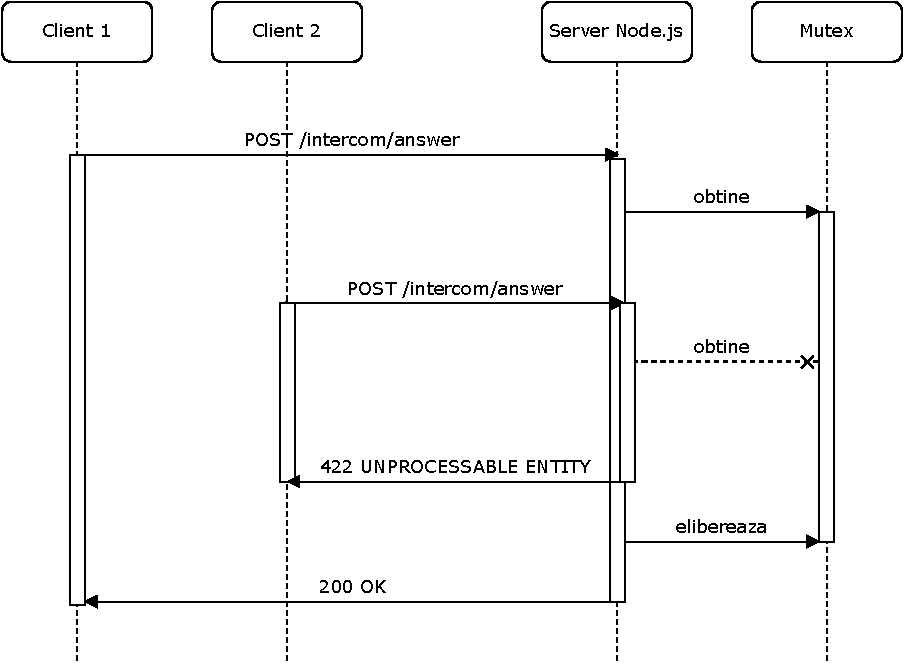
\includegraphics[width=0.6\textwidth]{04/03_mutex_diagram.pdf}  
  }
  \caption{Ilustrare resursa disputata intre doi utilizatori}
\end{figure}


\subsubsection {Validarea entitatilor}

Foloseste functii din Typescript si NestJS pentru a adauga si citi metadate prin intermediul decoratorilor de metode. \acrfull{dto} este reprezentarea unui model din baza de date, dar encodat favorbail pentru interpretarea usoara a clientilor. Majoritar, acesta va contine mai putine campuri decat exista in baza de date (reprezentarea unui utilizator nu va avea campul pentru parola).

Campurile unui \acrfull{dto} sunt adnotate cu tipul asteptat la runtime, si printr-un interceptor de nest care ruleaza atunci cand este invocata metoda unui controller \acrshort{rest}, obiectul primit ca parametru este verificat contra specificatiilor din metadate. In cazul in care validarea esueaza, clientului ii este intors status 400 (Bad Request) indicand o eroare de formatare a requestului.

Mutand responsabilitatea verificarii entitatilor in cadrul serverului, se mitigheaza si lipsa unei scheme la nivelul bazei de date, inerente solutiilor NoSQL. Prin urmare se reduce riscul unor inconsistente in datele stocate.

\subsubsection {Roluri}

Urmarind "reteta" de dezvoltare observata in validarea entitatilor, am creat un mecanism de adaugare a metadatelor pe rutele controllerelor despre ce roluri de user au acces sa le cheme.

Partea de verificare a unui user in timpul unui request, revine asa-numitelor "Guard-uri" care implementeaza o interfata comuna. In cazul vederilor pentru aplicatia de admin dormin sa restrictionam afisarea sa userilor normali, asadar inlantuim "Guard-urile" ce garanteaza autentificarea unui utilizator si rolul de administrator. In cazul in care un user nu este administrator, acestuia i se intoarce un cod de status 403 (Forbidden) - serverul a autentificat utilizatorul, dar acesta nu are suficiente permisiuni pentru a accesa resursa

\subsubsection {Documentatie}

Intr-un proiect de lunga durata, documentatia joaca un rol esential in usurinta de mentenanta si dezvoltare a codului. Despartirea logica a componentelor aplicatiei cat si explicarea eventualelor cai logice si raspunsuri posibile ajuta atat clientii externi consumatori ai \acrshort{api}-ului cat si dezvoltatorii noi care incearca sa introduca primele modificari.

Astfel, am ales Swagger pentru a parcurge proiectul si genera pagini de documentatie pentru toate rutele serviciului \acrshort{rest}, impreuna cu comentarii si potentialele status code-uri la care trebuie sa se astepte clientii. De asemenea, Swagger include si un client \acrshort{rest} in pagina, impreuna cu schema obiectelor si tipurile de date asteptate nu lasa loc de interpretat in comportamentul serverului.

\subsection {Android}

Android este o platforma mobile care s-a maturizat pe parcusul a 12 versiuni majore si principalul competitor de piata al iOS. Im dezvoltarea acestei aplicatii am folosit o abordare similara cu cea a serverului, fiind organizata intr-un pattern de design \acrshort{mvc}. De asemenea am folosit un framework pentru injectarea automata a dependintelelor.

\subsubsection {Dependency Injection}

Pentru a gestiona mai usor modulele aplicatiei si diferitele surse de date, am ales sa folosesc Dagger2, un framework bine cunoscut de Java. El vine cu extensii pentru Android ce permit controlul granular asupra instantierii modulelor necesare in functie de ciclul de viata al aplicatiei sau al unui Activity. Astfel putem defini module globale, precum cel care cheama api-ul web, instantiat o singura data pe durata aplicatiei, sau module locale, precum cel de SharedPreferences care se realoca de fiecare data cand se intra in ecranul principal.

Pe langa organizarea proiectului in module logice in functie de functionalitati, Dagger ajuta si la managementul memoriei intr-un limbaj de programare cu Garbage Collector, precum Java, evitand alocari nenecesare sau frecvente.


\section {Implementarea sistemului}

\subsubsection {Baza de date}

Schema documentelor mongo aici

\section {Testarea sistemului}

\subsection {Server}

Chiar daca NestJS ofera suport pentru scrierea de teste unitare prin adaugarea de fisere $.spec.ts$, cea mai mare provocare a fost mockuirea modulului care comunica cu pinii \acrshort{gpio} ai Raspberry Pi. Wrapperul de JavaScript comunica prin intermediul \acrfull{napi} cu o librarie statica ce realizeaza serializarea si deserializarea datelor dintre Node.js/V8 VM si C/C++. Aceasta librarie se linkeaza la randul ei cu $bcm2835$ pentru a obtine acces la pinii \acrshort{gpio} si alte functii din sistemul de Intrare/Iesire al cipului Broadcom 2835.

Astfel suntem prezentati cu o problema, libraria \acrshort{napi} poate fi compilata pe alte arhitecturi, dar cu siguranta va genera o exceptie la rulare cand va incerca sa execute instructiuni invalide. Este nevoie de o logica de control care sa permita rularea si returnarea unor date prestabilite, cand se detecteaza rularea pe o arhitectura invalida, cum ar fi in cazul testelor rulate in mod automat prin intermediul pipelineului de integrare continua.

\subsubsection {Teste unitare}

Urmatorul pas a fost elaborarea testelor unitare. Am ales sa creez un fisier $.spec.ts$ pentru fiecare controller al API-ului acoperind astfel intreaga functionalitate a aplicatiei. Pentru controllerului responsabil deschiderii interfonului am mockuit serviciile Firebase si baza de date, testand mecanismul de deschidere/inchidere a interfonului in cazul in care aceeasi resursa este accesata de mai multi utilizatori concomitent.

\subsubsection {Teste end-to-end}

Pentru a ne asigura ca serviciul \acrshort{rest} raspunde corect se impune necesitatea testelor cap coada, unde se instantiaza aplicatia intr-o maniera similara productiei, iar cu ajutorul unui client rest se trimit cereri prestabilite si se asteapta dupa raspunsurile lor. Astfel parcurgem toata logica serverului, cap-coada si ne vom asigura de un comportament predictibil.

\subsection {Aplicatie mobila}

Din cauza fragmentarii foarte mari a versiunilor si configuratiilor posibile pentru toate dispozitivele Android pe care ar putea rula aplicatia, am decis sa folosesc "Firebase Test Lab", un serviciu de la Google care ofera posibilitatea rularii unui test automat sau scriptat pe o gama larga de dispozitive. 
Asiguram astfel un minim control al calitatii prin descoperirea timpurie a exceptiilor netratate.

Tipul de test ales este cel "Robo", care va analizeaza inteligent interfata vizuala a aplicatiei, dupa care va genera evenimente de input ca si cum ar fi un utilizator. Planul "Spark" de la Firebase ne da acces la 5 rulari pe dispozitive fizice pe zi si 10 dispozitive virtuale, deci testele au fost executate in limita acestor constrangeri. 

Pentru a rula un testa, trebuie sa incarcam un APK sau un AAB, alegem dispozitivele pe care dorim sa testam si eventualii pasi aditionali pe care ii dorim acoperiti de Robo. Dupa introducerea id-ului pentru campurile de username si parola impreuna cu valorile asociate unui cont de test, a reusit sa se autentifice si sa faca un stress-test al aplicatiei.


De asemenea "Test Lab" poate fi chemat din interiorul pipelineul de integrare continua pentru a rula teste automat dupa terminarea unui build pe un anumit branch, verificand flow-uri exesitente din aplicatie impotriva potentialelor regresii aparute.